\documentclass{beamer}
\usepackage[T1]{fontenc}
\usepackage[utf8]{inputenc}
\usepackage{xcolor}
\usepackage{listings}
\usepackage{graphicx}
\usepackage{tikz}
\usepackage{amsmath}
\usepackage{algorithm}
\usepackage{algpseudocode}
\usepackage{bookmark}

\usetikzlibrary{shapes.geometric, arrows.meta, shadows, positioning}

% Theme
\usetheme{Madrid}
\usecolortheme{default}
\setbeamertemplate{navigation symbols}{}

% Custom JavaScript definition for listings
\lstdefinelanguage{JavaScript}{
  keywords={break, case, catch, continue, debugger, default, delete, do, else, false, finally, for, function, if, in, instanceof, new, null, return, switch, this, throw, true, try, typeof, var, void, while, with, as, async, await, const, let, class, export, import, from, extends},
  morecomment=[l]{//},
  morecomment=[s]{/*}{*/},
  morestring=[b]',
  morestring=[b]"
}

\lstset{
  language=JavaScript,
  basicstyle=\ttfamily\small,
  keywordstyle=\color{blue}\bfseries,
  commentstyle=\color{gray},
  stringstyle=\color{red},
  breaklines=true,
  showstringspaces=false
}

\title{DICOM Volume Visualization}
\subtitle{From Medical Imaging Data to Interactive 3D Rendering}
\author{Graphicus-Harena Project}
\date{\today}

\begin{document}
%============================
% TITLE SLIDE
%============================
\frame{\titlepage}

%============================
% TABLE OF CONTENTS
%============================
\begin{frame}
\frametitle{Overview}
\tableofcontents
\end{frame}

%============================
% SECTION 1: INTRODUCTION
%============================
\section{Introduction}

\begin{frame}
\frametitle{What is DICOM?}
\begin{itemize}
  \item \textbf{DICOM} = Digital Imaging and Communications in Medicine
  \item Standard format for medical imaging data
  \item Contains both metadata and pixel data
  \item Common in CT, MRI, X-ray, and other modalities
  \item Multiple files form a 3D volume (one file per slice)
\end{itemize}

\vspace{1cm}

\textbf{Goal:} Build an interactive web-based viewer that:
\begin{enumerate}
  \item Reads multiple DICOM files
  \item Constructs a 3D volume data structure
  \item Renders orthogonal slices (axial, sagittal, coronal)
  \item Uses WebGL for GPU-accelerated rendering
\end{enumerate}
\end{frame}

% Ensure these are in your preamble:
% \usetikzlibrary{positioning, arrows.meta, shadows}

\begin{frame}[fragile]
\frametitle{Architecture Overview}
\begin{center}
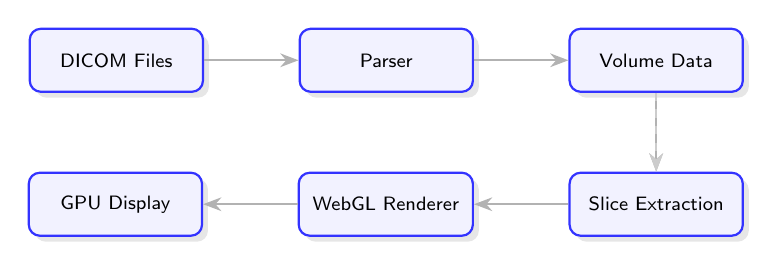
\begin{tikzpicture}[
    % Reduced horizontal (1.2cm) and vertical (1.0cm) spacing
    node distance=1.0cm and 1.2cm,
    force/.style={
        rectangle, rounded corners, draw=blue!80, fill=blue!5, 
        thick, inner sep=5pt, text centered, 
        minimum width=2.2cm, % Slightly narrower boxes
        minimum height=0.8cm,
        drop shadow={opacity=0.2}, 
        font=\sffamily\scriptsize % Smaller font to save space
    },
    arrow/.style={-Stealth, thick, draw=gray!60}
]
  % Top Row: Ingestion
  \node[force] (dicom) {DICOM Files};
  \node[force, right=of dicom] (parser) {Parser};
  \node[force, right=of parser] (volume) {Volume Data};
  
  % Bottom Row: Rendering
  \node[force, below=of volume] (slices) {Slice Extraction};
  \node[force, left=of slices] (webgl) {WebGL Renderer};
  \node[force, left=of webgl] (display) {GPU Display};

  % Connecting Arrows
  \draw[arrow] (dicom) -- (parser);
  \draw[arrow] (parser) -- (volume);
  \draw[arrow] (volume) -- (slices);
  \draw[arrow] (slices) -- (webgl);
  \draw[arrow] (webgl) -- (display);

  % Optional: Visual flow indicator
  \draw[arrow, dashed, color=gray!40] (volume.south) -- (slices.north);

\end{tikzpicture}
\end{center}

\begin{exampleblock}{Key Stages}
\begin{itemize}
    \item \textbf{Data:} Normalizing diverse DICOM tags into a consistent voxel grid.
    \item \textbf{Compute:} Leveraging WebGL for hardware-accelerated interpolation.
\end{itemize}
\end{exampleblock}
\end{frame}
%============================
% SECTION 2: DICOM PARSING
%============================
\section{Reading DICOM Data}

\begin{frame}
\frametitle{DICOM File Structure}
DICOM files are binary with tagged structure:

\begin{itemize}
  \item \textbf{Group and Element tags}: (XXXX, XXXX) in hexadecimal
  \item \textbf{Value Representation (VR)}: Data type (UI, CS, LO, US, OW, etc.)
  \item \textbf{Length}: Bytes in the value
  \item \textbf{Value}: Actual data
\end{itemize}

\vspace{0.5cm}

\textbf{Key DICOM Tags for Image Slices:}
\small
\begin{tabular}{|l|l|}
\hline
\textbf{Tag} & \textbf{Description} \\
\hline
(0028,0010) & Rows (height) \\
(0028,0011) & Columns (width) \\
(0028,0100) & Bits Allocated (8 or 16) \\
(0020,0013) & Instance Number \\
(0020,0032) & Image Position Patient (x, y, z) \\
(7FE0,0010) & Pixel Data (binary image) \\
\hline
\end{tabular}
\end{frame}

\begin{frame}[fragile]{DICOM Parsing: Metadata}
\begin{columns}
\begin{column}{0.5\textwidth}
\begin{lstlisting}
// Extract Header Tags
const rows = dataSet.uint16('x00280010');
const cols = dataSet.uint16('x00280011');
const bits = dataSet.uint16('x00280100');
\end{lstlisting}
\end{column}
\begin{column}{0.5\textwidth}
\small
\textbf{Key Tags:}
\begin{itemize}
    \item \texttt{x00280010}: Image Height (Rows)
    \item \texttt{x00280011}: Image Width (Columns)
    \item \texttt{x00280100}: Bits Allocated (usually 16-bit for CT/MRI)
\end{itemize}
\end{column}
\end{columns}
\end{frame}

\begin{frame}[fragile]{DICOM Parsing: Pixel Data}
\begin{lstlisting}
// Locate the Pixel Data Element (7FE0,0010)
const pixelElement = dataSet.elements.x7fe00010;

// Create a view without copying the underlying buffer
const pixelData = new Uint16Array(
  byteArray.buffer, 
  pixelElement.dataOffset, 
  pixelElement.length / 2
);
\end{lstlisting}
\vfill
\begin{alertblock}{Performance Note}
Using \texttt{Uint16Array} on the existing \texttt{buffer} prevents a full memory copy, which is critical when loading 500+ slices.
\end{alertblock}
\end{frame}

\begin{frame}[fragile]{DICOM Parsing: Spatial Context}
\begin{lstlisting}
// Image Position (Patient) Tag
const posStr = dataSet.string('x00200032');
const [x, y, z] = posStr.split(' ').map(Number);
\end{lstlisting}
\vfill
\begin{itemize}
    \item \textbf{Image Position (Patient):} Specifies the $x, y, z$ coordinates of the upper left hand corner of the slice.
    \item \textbf{Stacking:} We use the \texttt{z} value to sort slices into a coherent 3D volume.
\end{itemize}
\end{frame}

\begin{frame}
\frametitle{Data Type Handling}
\begin{itemize}
  \item \textbf{8-bit images}: Uint8Array (common in radiography)
  \item \textbf{16-bit images}: Uint16Array (common in CT/MRI)
  \item \textbf{Byte ordering}: Little-endian on most systems
  \item \textbf{Pixel representation}: Usually unsigned (0 to max)
  \item Hounsfield Units in CT: Requires proper windowing
\end{itemize}

\vspace{0.5cm}

\textbf{Slice Collection:}
\begin{itemize}
  \item Multiple DICOM files $\rightarrow$ one file per slice
  \item Files must be sorted by spatial position
  \item Use \texttt{ImagePositionPatient} (most reliable)
  \item Fallback to \texttt{InstanceNumber}
\end{itemize}
\end{frame}
%============================
% SECTION 3: VOLUME DATA STRUCTURE
%============================
\section{Volume Data Structure}

\begin{frame}
\frametitle{Volume Representation}

\textbf{Definition:} A 3D array of voxel values organized as:
$$\text{Volume}[z][y][x] = \text{pixel intensity}$$

\begin{itemize}
  \item \textbf{Dimensions}: width $\times$ height $\times$ depth
  \item \textbf{Spacing}: Physical distance between voxels
  \item \textbf{Storage}: Linear Float32Array (memory efficient)
  \item \textbf{Indexing}: $(x, y, z) \rightarrow \text{offset} = x + y \cdot W + z \cdot W \cdot H$
\end{itemize}

\vspace{0.5cm}

\textbf{Key Properties:}
\begin{itemize}
  \item width: Number of columns
  \item height: Number of rows
  \item depth: Number of slices
  \item spacing: [pixelSpacing.x, pixelSpacing.y, sliceThickness]
  \item data: Float32Array (normalized pixel values)
  \item minValue, maxValue: For windowing
\end{itemize}
\end{frame}

\begin{frame}[fragile]{Volume Construction: Memory Mapping}
To pass data to a \textbf{WebGL 3D Texture}, we must flatten our stack of 2D slices into a single 1D array.

\begin{block}{Indexing Formula}
The position of a voxel at $(x, y, z)$ in the linear buffer is:
\[ \text{Index} = (z \times \text{width} \times \text{height}) + (y \times \text{width}) + x \]
\end{block}

\begin{lstlisting}
// Allocate linear array for the entire volume
this.data = new Float32Array(
  this.width * this.height * this.depth
);

// z-plane offset in the 1D array
const planeOffset = z * this.width * this.height;
\end{lstlisting}

\vfill
\small \textit{Note: We use \texttt{Float32Array} to allow for Hounsfield Unit (HU) precision after normalization.}
\end{frame}

\begin{frame}[fragile]{Volume Construction: Normalization}
The final step, \texttt{computeMinMax()}, is critical for rendering contrast.

\begin{lstlisting}
computeMinMax() {
  let min = Infinity, max = -Infinity;
  for (let i = 0; i < this.data.length; i++) {
    const val = this.data[i];
    if (val < min) min = val;
    if (val > max) max = val;
  }
  this.stats = { min, max };
}
\end{lstlisting}

\begin{itemize}
    \item \textbf{Windowing:} Allows the user to focus on "Soft Tissue" vs "Bone".
    \item \textbf{GPU Ready:} Pre-calculating these bounds allows the shader to normalize values on the fly: $v_{norm} = \frac{v - min}{max - min}$.
\end{itemize}
\end{frame}

\begin{frame}[fragile]
\frametitle{Memory Layout: 3D to 1D Mapping}

\begin{center}
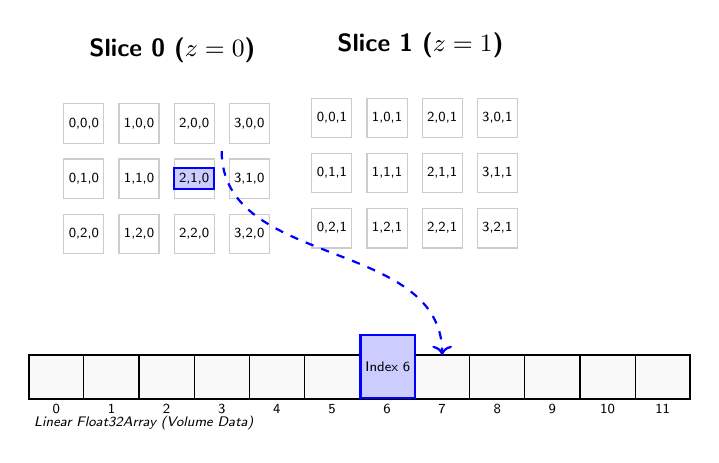
\begin{tikzpicture}[
    scale=0.7, 
    z={(0.5cm,0.4cm)}, % Custom 3D perspective
    node font=\tiny\sffamily,
    cell/.style={draw=black!20, fill=white, minimum size=0.5cm},
    highlight/.style={fill=blue!20, draw=blue, thick}
]

  % --- SLICE 1 (Back/z=1) ---
  \begin{scope}[shift={(2.5,-1.5,4)}]
    \node[anchor=south west, font=\bfseries\small] at (0,3) {Slice 1 ($z=1$)};
    \foreach \y in {0,...,2}
      \foreach \x in {0,...,3}
        \node[cell] (z1-\x-\y) at (\x,2-\y) {\x,\y,1};
  \end{scope}

  % --- SLICE 0 (Front/z=0) ---
  \begin{scope}[shift={(0,0,0)}]
    \node[anchor=south west, font=\bfseries\small] at (0,3) {Slice 0 ($z=0$)};
    \foreach \y in {0,...,2}
      \foreach \x in {0,...,3}
        \node[cell] (z0-\x-\y) at (\x,2-\y) {\x,\y,0};
        
    % Highlight a specific voxel: (2,1,0)
    \node[highlight] at (2,1) {2,1,0};
  \end{scope}

  % --- LINEAR ARRAY (Below) ---
  \begin{scope}[shift={(-1,-3,0)}]
    \draw[thick, fill=gray!5] (0,0) rectangle (12,0.8);
    \foreach \i in {0,...,11} {
        \draw (\i,0) -- (\i,0.8);
        \node[anchor=north] at (\i+0.5, 0) {\i};
    }
    % Highlight the mapped index: 2 + (1*4) + (0*12) = 6
    \node[highlight, minimum height=0.8cm, anchor=south west] at (6,0) {Index 6};
    \node[anchor=north west, font=\itshape] at (0,-0.2) {Linear Float32Array (Volume Data)};
  \end{scope}

  % Connection Arrow
  \draw[->, blue, thick, dashed] (2.5,1.5,0) [out=-90, in=90] to (6.5,-2.2,0);

\end{tikzpicture}
\end{center}

\begin{exampleblock}{The Mapping Formula}
\[ \text{Index} = x + (y \cdot W) + (z \cdot W \cdot H) \]
\textbf{Calculation:} For $V(2,1,0) \rightarrow 2 + (1 \cdot 4) + (0 \cdot 12) = \mathbf{6}$
\end{exampleblock}

\end{frame}
%============================
% SECTION 4: SLICE EXTRACTION
%============================
\section{Slice Extraction}

\begin{frame}
\frametitle{Orthogonal Slices in Medical Imaging}

\begin{center}
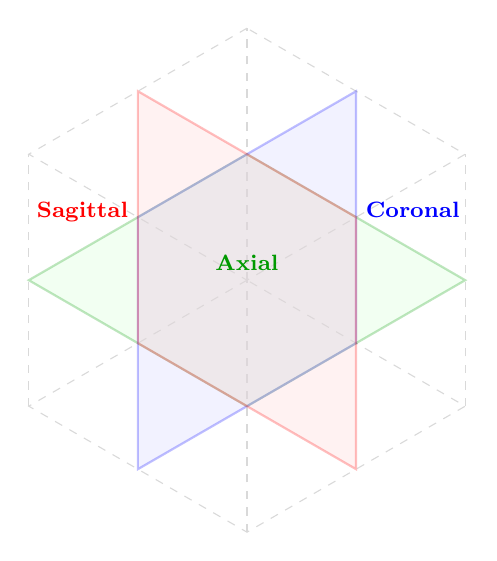
\begin{tikzpicture}[
    scale=1.6, 
    % Manual Isometric Projection:
    x={(-0.866cm,-0.5cm)}, y={(0.866cm,-0.5cm)}, z={(0cm,1cm)},
    plane/.style={opacity=0.25, thick, draw}
]
  % 3D volume cube (Bounding Box)
  \draw[gray!30, dashed] (0,0,0) -- (2,0,0) -- (2,2,0) -- (0,2,0) -- cycle;
  \draw[gray!30, dashed] (0,0,2) -- (2,0,2) -- (2,2,2) -- (0,2,2) -- cycle;
  \draw[gray!30, dashed] (0,0,0) -- (0,0,2) (2,0,0) -- (2,0,2) (2,2,0) -- (2,2,2) (0,2,0) -- (0,2,2);
  
  % Axial Plane (Z = 1) - Green
  \draw[plane, color=green!60!black, fill=green!20] (0,0,1) -- (2,0,1) -- (2,2,1) -- (0,2,1) -- cycle;

  % Coronal Plane (Y = 1) - Blue
  \draw[plane, color=blue, fill=blue!20] (0,1,0) -- (2,1,0) -- (2,1,2) -- (0,1,2) -- cycle;
  
  % Sagittal Plane (X = 1) - Red
  \draw[plane, color=red, fill=red!20] (1,0,0) -- (1,2,0) -- (1,2,2) -- (1,0,2) -- cycle;
  
  % Labels with subtle positioning
  \node[red, font=\bfseries\footnotesize, anchor=north east] at (1,0,1.2) {Sagittal};
  \node[blue, font=\bfseries\footnotesize, anchor=north west] at (0,1,1.2) {Coronal};
  \node[green!60!black, font=\bfseries\footnotesize, anchor=south] at (1,1,1) {Axial};

\end{tikzpicture}
\end{center}

\vspace{-0.2cm}
\begin{columns}[T]
  \begin{column}{0.3\textwidth}
    \centering \textcolor{red}{\textbf{Sagittal}} \\ \scriptsize $x$ = constant \\ (YZ Plane)
  \end{column}
  \begin{column}{0.3\textwidth}
    \centering \textcolor{blue}{\textbf{Coronal}} \\ \scriptsize $y$ = constant \\ (XZ Plane)
  \end{column}
  \begin{column}{0.3\textwidth}
    \centering \textcolor{green!60!black}{\textbf{Axial}} \\ \scriptsize $z$ = constant \\ (XY Plane)
  \end{column}
\end{columns}
\end{frame}

\begin{frame}[fragile]
\frametitle{Extracting Axial Slices}
\begin{lstlisting}
  const out = new Uint8Array(w * h);
  const z = Math.max(0, Math.min(depth - 1, index));
  const offset = z * w * h;
  const range = this.maxValue - this.minValue;

  for (let i = 0; i < w * h; i++) {
    // Linear normalization: [min, max] -> [0, 255]
    const norm = (this.data[offset + i] - this.minValue) / range;
    out[i] = Math.round(norm * 255);
  }
  return { data: out, width: w, height: h };
\end{lstlisting}
\begin{block}{Efficiency}
Axial slices are the fastest to extract because they correspond to a contiguous block of memory in our linear array.
\end{block}
\end{frame}

\begin{frame}[fragile]
\frametitle{Improving Contrast: Windowing}
To see bone or soft tissue specifically, we apply a linear transform based on a \textbf{Center} ($C$) and \textbf{Width} ($W$):

\begin{lstlisting}
const low = center - width / 2;
const high = center + width / 2;

// Inside the loop:
let val = this.data[offset + i];
let normalized = (val - low) / (high - low);
out[i] = Math.max(0, Math.min(255, normalized * 255));
\end{lstlisting}

\begin{table}
\small
\centering
\begin{tabular}{lrr}
\hline
\textbf{Tissue} & \textbf{Center (L)} & \textbf{Width (W)} \\ \hline
Bone            & +400               & 1500               \\
Soft Tissue     & +50                & 400                \\
Lung            & -600               & 1500               \\ \hline
\end{tabular}
\end{table}
\end{frame}

\begin{frame}[fragile]
\frametitle{Extracting Sagittal Slices (X-Plane)}
\begin{lstlisting}
  const out = new Uint8Array(D * H); // z x y
  const x = Math.max(0, Math.min(W - 1, index));
  for (let y = 0; y < H; y++) {
    const yOffset = y * W; // Row offset
    for (let z = 0; z < D; z++) {
      // Manual Indexing: x + yW + zWH
      const volumeIdx = x + yOffset + (z * W * H);
      const voxel = this.data[volumeIdx];
      const outIdx = y * D + z;
      out[outIdx] = ((voxel - min) / range) * 255;
    }
  }
  return { data: out, width: D, height: H };
\end{lstlisting}

\begin{alertblock}{Performance Challenge: Non-Contiguous Access}
Unlike Axial slices, Sagittal voxels are separated by exactly \texttt{width} elements (for $y$) and \texttt{width * height} elements (for $z$). This results in poor \textbf{cache locality}.
\end{alertblock}
\end{frame}

\begin{frame}[fragile]
\frametitle{Extracting Coronal Slices (Y-Plane)}
\begin{lstlisting}
  const out = new Uint8Array(D * W); // z x x
  const y = Math.max(0, Math.min(H - 1, index));
  const yOffset = y * W; // Constant row offset
  for (let x = 0; x < W; x++) {
    for (let z = 0; z < D; z++) {
      // Indexing: x + (y-const) + z*(W*H)
      const volumeIdx = x + yOffset + (z * W * H);
      const outIdx = x * D + z;
      const voxel = this.data[volumeIdx];
      out[outIdx] = ((voxel - min) / range) * 255;
    }
  }
  return { data: out, width: D, height: W };
\end{lstlisting}

\begin{block}{Memory Access Pattern}
The Coronal plane samples voxels that are exactly $W \cdot H$ units apart in the linear array for each $z$ step.
\end{block}
\end{frame}

\begin{frame}
\frametitle{Slice Extraction Complexity}

\textbf{Time Complexity:}
\begin{itemize}
  \item Axial: $O(W \times H)$ - single plane lookup
  \item Sagittal: $O(W \times D)$ - multiple lookups
  \item Coronal: $O(W \times D)$ - multiple lookups
\end{itemize}

\vspace{0.5cm}

\textbf{Normalization:}
\begin{itemize}
  \item Convert float voxels to 8-bit grayscale
  \item Compute min/max during volume construction
  \item Apply linear mapping:
  $$\text{output} = \frac{\text{voxel} - \text{min}}{\text{max} - \text{min}} \times 255$$
  \item Enables proper visualization of contrast
\end{itemize}
\end{frame}
%============================
% CHAPTER 5: WEBGL RENDERING
%============================
\section{WebGL Rendering: GPU-Powered Visualization}

\begin{frame}
\frametitle{Chapter 5: Awakening the GPU}

\begin{columns}[T]
\begin{column}{0.6\textwidth}
  \textbf{Dr. Chen's Realization:} "JavaScript alone can't render 50 million voxels at 60 FPS. I need the GPU!"
  
  \vspace{0.5cm}
  \textbf{WebGL} is the bridge between JavaScript and GPU hardware:
  \begin{itemize}
    \item \textbf{JavaScript}: Handles data loading and logic
    \item \textbf{WebGL API}: GPU resource management
    \item \textbf{Shaders}: GPU programs for rendering
    \item \textbf{Canvas}: Display output
  \end{itemize}
\end{column}
\begin{column}{0.35\textwidth}
  \begin{center}
    \begin{tikzpicture}[scale=0.8]
      % GPU pipeline
      \draw[fill=medicalblue!20, rounded corners] (0,0) rectangle (2,0.5);
      \node[medicalblue] at (1,0.25) {JavaScript};
      
      \draw[fill=softgreen!30, rounded corners] (0,0.7) rectangle (2,1.2);
      \node[medicalgreen] at (1,0.95) {WebGL API};
      
      \draw[fill=medicalred!20, rounded corners] (0,1.4) rectangle (2,1.9);
      \node[medicalred] at (1,1.65) {GPU Shaders};
      
      \draw[fill=softblue!30, rounded corners] (0,2.1) rectangle (2,2.6);
      \node[medicalblue] at (1,2.35) {Canvas Display};
      
      % Arrows
      \draw[->, thick] (1,0.5) -- (1,0.7);
      \draw[->, thick] (1,1.2) -- (1,1.4);
      \draw[->, thick] (1,1.9) -- (1,2.1);
    \end{tikzpicture}
    \vspace{0.3cm}
    {\small\color{medicalgray}WebGL Pipeline}
  \end{center}
\end{column}
\end{columns}

\knowledgecheck{GPU vs CPU}
Why can't we render medical volumes using only JavaScript? What specific advantages does the GPU provide?
\end{frame}

\begin{frame}{WebGL Pipeline: GPU Resources}
\begin{center}
\begin{tikzpicture}[
    node distance=1cm,
    res/.style={rectangle, rounded corners, draw=medicalblue!60!black, fill=softblue!20, thick, text width=2.8cm, align=center, font=\sffamily\small, minimum height=1cm}
]
  \node[res] (tex) {3D Texture \\ \scriptsize (Voxel Data)};
  \node[res, left=of tex] (buf) {Geometry Buffers \\ \scriptsize (Quad Vertices)};
  \node[res, right=of tex] (shd) {Shader Source \\ \scriptsize (GLSL Code)};

  \draw[dashed, medicalgray] (-5, -1) -- (5, -1) node[midway, below, font=\tiny] {Uploaded from CPU to GPU VRAM};
\end{tikzpicture}
\end{center}

\begin{block}{Volume Storage}
The entire 3D DICOM stack is stored as a \textbf{Texture3D}, allowing the GPU to perform hardware-accelerated interpolation between slices.
\end{block}

\clinicalexample{GPU Memory}
A 512×512×200 CT volume requires ~200MB of GPU memory. Modern GPUs can handle this, but memory management is critical.
\end{frame}

\begin{frame}{WebGL Pipeline: Shader Execution}
\begin{center}
\begin{tikzpicture}[
    node distance=1.2cm,
    pipe/.style={rectangle, rounded corners, draw=medicalgreen!60!black, fill=softgreen!20, thick, text width=3.5cm, align=center, font=\sffamily\small, minimum height=0.9cm},
]
  \node[pipe] (vs) {Vertex Shader \\ \scriptsize (Positions the Quad)};
  \node[pipe, below=of vs] (fs) {Fragment Shader \\ \scriptsize (Samples Texture)};
  \node[pipe, below=of fs] (canvas) {Canvas Display \\ \scriptsize (Final Output)};

  \draw[-Stealth, thick, medicalgray] (vs) -- (fs);
  \draw[-Stealth, thick, medicalgray] (fs) -- (canvas);
\end{tikzpicture}
\end{center}

\begin{itemize}
    \item \textbf{Rasterization:} The GPU determines which pixels on screen cover the geometry (our slice quad).
    \item \textbf{Texture Sampling:} For every fragment, the shader samples the 2D texture to get the grayscale value.
\end{itemize}

\knowledgecheck{Shader Roles}
What does the vertex shader do? What does the fragment shader do? Why do we need both?
\end{frame}

\begin{frame}[fragile]
\frametitle{WebGL Context Initialization}

\begin{lstlisting}
constructor(canvas: HTMLCanvasElement, 
            vertexSource: string, 
            fragmentSource: string) {
  this.canvas = canvas;
  
  // Get WebGL context
  const gl = canvas.getContext('webgl');
  if (!gl) throw new Error('WebGL not supported');
  
  this.gl = gl;
  
  // Enable depth testing
  this.gl.enable(this.gl.DEPTH_TEST);
  this.gl.depthFunc(this.gl.LEQUAL);
  
  // Set viewport
  this.gl.viewport(0, 0, canvas.width, canvas.height);
  
  // Compile shaders
  this.program = new ShaderProgram(gl, 
                                   vertexSource, 
                                   fragmentSource);
  
  // Create camera and controls
  this.camera = new Camera();
  this.mouse = new MouseController(canvas, this.camera);
}
\end{lstlisting}
\end{frame}

\begin{frame}
\frametitle{Shader Program Compilation}

\textbf{Pipeline:}
\begin{enumerate}
  \item \textbf{Create Shader}: \texttt{gl.createShader(type)}
  \item \textbf{Set Source}: \texttt{gl.shaderSource(shader, source)}
  \item \textbf{Compile}: \texttt{gl.compileShader(shader)}
  \item \textbf{Create Program}: \texttt{gl.createProgram()}
  \item \textbf{Attach Shaders}: \texttt{gl.attachShader(program, shader)}
  \item \textbf{Link}: \texttt{gl.linkProgram(program)}
  \item \textbf{Use}: \texttt{gl.useProgram(program)}
\end{enumerate}

\vspace{0.5cm}

\textbf{Error Handling:}
\begin{itemize}
  \item Check \texttt{gl.COMPILE\_STATUS} after compilation
  \item Check \texttt{gl.LINK\_STATUS} after linking
  \item Use \texttt{getShaderInfoLog()} for debug messages
\end{itemize}
\end{frame}

\begin{frame}[fragile]
\frametitle{Vertex Shader Example}

\textbf{Purpose:} Transform geometry to screen space

\begin{lstlisting}[language=glsl]
attribute vec3 a_position; // Vertex position
attribute vec2 a_texcoord; // Texture coordinate
varying vec2 v_texcoord;   // To fragment shader
uniform mat4 u_matrix;     // Model-view-projection

void main() {
  // Pass texture coordinate to fragment shader
  v_texcoord = a_texcoord;
  // Transform position
  gl_Position = u_matrix * vec4(a_position, 1.0);
}
\end{lstlisting}

\textbf{Key Concepts:}
\begin{itemize}
  \item \textbf{attribute}: Per-vertex data
  \item \textbf{uniform}: Constant for all vertices
  \item \textbf{varying}: Interpolated per fragment
  \item \textbf{gl\_Position}: Output vertex position
\end{itemize}
\end{frame}

\begin{frame}[fragile]
\frametitle{Fragment Shader Example}

\textbf{Purpose:} Determine color for each pixel

\begin{lstlisting}[language=glsl]
precision mediump float;
varying vec2 v_texcoord;
uniform sampler2D u_texture;

void main() {
  // Sample texture at this fragment
  float v = texture2D(u_texture, v_texcoord).r;
  
  // Convert to grayscale color
  gl_FragColor = vec4(v, v, v, 1.0);
}
\end{lstlisting}

\textbf{Key Concepts:}
\begin{itemize}
  \item \textbf{sampler2D}: 2D texture unit
  \item \textbf{texture2D()}: Sample texture at UV coords
  \item \textbf{gl\_FragColor}: Output pixel color
  \item \textbf{precision}: Floating-point precision
\end{itemize}
\end{frame}

\begin{frame}[fragile,allowframebreaks]
\frametitle{Textures in WebGL}

\textbf{Texture Creation:}
\begin{itemize}
  \item \texttt{gl.createTexture()}: Allocate texture object
  \item \texttt{gl.bindTexture(gl.TEXTURE\_2D, tex)}: Bind for operations
  \item \texttt{gl.texImage2D()}: Upload pixel data
  \item \texttt{gl.texParameteri()}: Set filtering/wrapping
\end{itemize}

\vspace{0.3cm}

\textbf{Slice Texture Update:}
\begin{lstlisting}[language=JavaScript, basicstyle=\small\ttfamily]
// Create texture from slice data
gl.bindTexture(gl.TEXTURE_2D, this.sliceTexture);
gl.texImage2D(
  gl.TEXTURE_2D, 0, gl.LUMINANCE,
  width, height, 0,
  gl.LUMINANCE, gl.UNSIGNED_BYTE,
  sliceBytes
);
\end{lstlisting}

\vspace{0.3cm}

\textbf{Key Parameters:}
\begin{itemize}
  \item \textbf{LUMINANCE}: Single channel (grayscale). Perfect for DICOM!
  \item \textbf{UNSIGNED\_BYTE}: 8-bit values ($0-255$).
  \item \textbf{FILTERING}: \texttt{gl.LINEAR} allows the GPU to interpolate between pixels for smooth zooming.
\end{itemize}
\end{frame}

\begin{frame}
\frametitle{Vertex Buffers and Attributes}

\textbf{Vertex Buffer Object (VBO):}
\begin{itemize}
  \item GPU memory object storing vertex data
  \item \texttt{gl.createBuffer()}: Create buffer
  \item \texttt{gl.bindBuffer()}: Bind for operations
  \item \texttt{gl.bufferData()}: Upload data to GPU
\end{itemize}

\vspace{0.5cm}

\textbf{Vertex Attribute Pointers:}
\begin{itemize}
  \item \texttt{gl.enableVertexAttribArray()}: Enable attribute
  \item \texttt{gl.vertexAttribPointer()}: Describe layout
  \item \textbf{Parameters}: Index, size, type, normalized, stride, offset
\end{itemize}

\vspace{0.5cm}

\textbf{Example:} Position (vec3) + TexCoord (vec2)
\begin{itemize}
  \item Stride: $3 \times 4 + 2 \times 4 = 20$ bytes
  \item Offset for texcoord: $3 \times 4 = 12$ bytes
\end{itemize}
\end{frame}

\begin{frame}[fragile,allowframebreaks]
\frametitle{Rendering Loop}

\begin{lstlisting}
start(): void {
  const loop = () => {
    // Clear buffers
    this.gl.clear(this.gl.COLOR_BUFFER_BIT | 
                  this.gl.DEPTH_BUFFER_BIT);
    
    // Render scene
    if (this.mesh) {
      this.program.use();
      this.renderMesh(this.mesh);
    }
    
    // Render slices
    if (this.volume) {
      this.sliceProgram.use();
      this.renderSlices();
    }
    
    // Request next frame
    this.animationId = requestAnimationFrame(loop);
  };
  
  this.animationId = requestAnimationFrame(loop);
}
\end{lstlisting}

\textbf{Key Points:}
\begin{itemize}
  \item \textbf{requestAnimationFrame}: Browser-optimized rendering
  \item \textbf{Clear}: Remove previous frame data
  \item \textbf{Use}: Activate shader program
  \item \textbf{Draw}: Render geometry
\end{itemize}
\end{frame}

\begin{frame}
\frametitle{Depth Testing}

\textbf{Problem:} Overlapping geometry renders incorrectly without depth info

\vspace{0.5cm}

\textbf{Solution:} Depth Test (Z-buffering)
\begin{itemize}
  \item Each pixel stores depth value (distance from camera)
  \item Only draw pixel if new depth $<$ stored depth
  \item Ensures correct occlusion ordering
  \item \texttt{gl.enable(gl.DEPTH\_TEST)}
  \item \texttt{gl.depthFunc(gl.LEQUAL)}: Update if less or equal
\end{itemize}

\vspace{0.5cm}

\textbf{Configuration:}
\begin{itemize}
  \item \texttt{NEVER}: Never pass
  \item \texttt{LESS}: Pass if new $<$ stored
  \item \texttt{EQUAL}: Pass if equal
  \item \texttt{LEQUAL}: Pass if $\leq$ (typical)
  \item \texttt{GREATER}: Pass if $>$
  \item \texttt{ALWAYS}: Always pass
\end{itemize}
\end{frame}

\begin{frame}[fragile]
\frametitle{Matrix Transformations}

\textbf{Model-View-Projection (MVP) Matrix:}
$$\text{gl\_Position} = P \times V \times M \times \text{position}$$

Where:
\begin{itemize}
  \item $M$: Model matrix (geometry to world space)
  \item $V$: View matrix (world to camera space)
  \item $P$: Projection matrix (camera to screen space)
\end{itemize}

\vspace{0.5cm}

\textbf{Camera Implementation:}
\begin{itemize}
  \item Spherical coordinates: azimuth, polar, distance
  \item Eye position: $(r \sin\phi \cos\theta, r \sin\phi \sin\theta, r \cos\phi)$
  \item Look-at: Compute view matrix from eye, center, up
  \item Perspective: Configurable FOV, aspect ratio, near/far planes
\end{itemize}
\end{frame}
%============================
% SECTION 6: SLICE RENDERING
%============================
\section{Interactive Slice Rendering}

\begin{frame}
\frametitle{Textured Quad Rendering}

\textbf{Approach:} Render 2D slice as textured quad in 3D space

\begin{center}
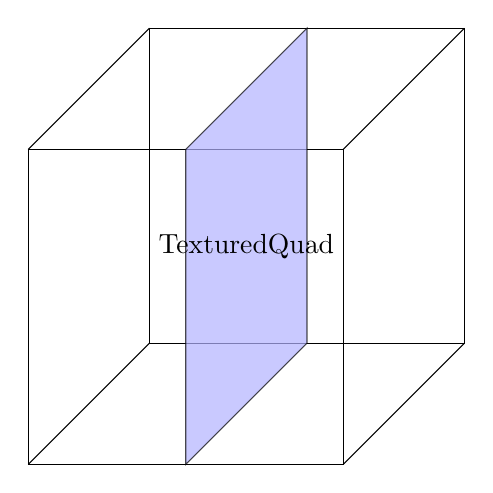
\begin{tikzpicture}[scale=2]
  % 3D volume
  \draw (0,0,0) -- (2,0,0) -- (2,2,0) -- (0,2,0) -- cycle;
  \draw (0,0,2) -- (2,0,2) -- (2,2,2) -- (0,2,2) -- cycle;
  \draw (0,0,0) -- (0,0,2);
  \draw (2,0,0) -- (2,0,2);
  \draw (2,2,0) -- (2,2,2);
  \draw (0,2,0) -- (0,2,2);
  
  % Textured quad
  \draw[fill=blue!30, opacity=0.7] (1,0,0) -- (1,2,0) -- (1,2,2) -- (1,0,2) -- cycle;
  \node at (1, 1, 1) {Textured\\Quad};
\end{tikzpicture}
\end{center}

\begin{itemize}
  \item Extract 2D slice from volume
  \item Create texture from slice data
  \item Position quad in 3D space (perpendicular to axis)
  \item Apply texture and render
\end{itemize}
\end{frame}

\begin{frame}[fragile]
\frametitle{Slice Texture Update}

\begin{lstlisting}
updateSliceTextureFromVolume(
  axis: 'axial' | 'sagittal' | 'coronal',
  index: number
) {
  // Extract 2D slice from volume
  const slice = this.volume.getSliceUint8(axis, index);
  
  // Create or update texture
  if (!this.sliceTexture) {
    this.sliceTexture = this.gl.createTexture();
  }
  
  this.gl.bindTexture(this.gl.TEXTURE_2D, this.sliceTexture);
  
  // Upload slice data as texture
  this.gl.texImage2D(
    this.gl.TEXTURE_2D, 0, this.gl.LUMINANCE,
    slice.width, slice.height, 0,
    this.gl.LUMINANCE, this.gl.UNSIGNED_BYTE,
    slice.data
  );
  
  // Set texture parameters
  this.gl.texParameteri(this.gl.TEXTURE_2D, 
    this.gl.TEXTURE_MIN_FILTER, this.gl.LINEAR);
  this.gl.texParameteri(this.gl.TEXTURE_2D, 
    this.gl.TEXTURE_MAG_FILTER, this.gl.LINEAR);
}
\end{lstlisting}
\end{frame}

\begin{frame}[fragile]
\frametitle{Quad Geometry Creation}

\begin{lstlisting}
updateSliceMesh(axis: 'axial' | 'sagittal' | 'coronal', 
                index: number) {
  
  let positions: number[] = [];
  let texcoords: number[] = [];
  
  if (axis === 'axial') {
    // Quad at z = index, spans x and y
    const z = this.indexToWorldZ(index);
    const minX = 0, maxX = 1;
    const minY = 0, maxY = 1;
    
    positions = [
      minX, minY, z,  // bottom-left
      maxX, minY, z,  // bottom-right
      minX, maxY, z,  // top-left
      maxX, maxY, z   // top-right
    ];
    
    texcoords = [
      0, 0,  // UV mapping
      1, 0,
      0, 1,
      1, 1
    ];
  }
  // Similar for sagittal and coronal...
  
  // Update GPU buffers
  this.updateGeometryBuffers(positions, texcoords);
}
\end{lstlisting}
\end{frame}

\begin{frame}
\frametitle{Real-time Interaction}

\textbf{Slice Selection via Widgets:}

\begin{center}
\includegraphics[width=0.9\textwidth]{../assets/slice-control.png}
\end{center}

\begin{itemize}
  \item Slider for axial index: 0 to depth-1
  \item Slider for sagittal index: 0 to width-1
  \item Slider for coronal index: 0 to height-1
  \item onChange: Update slice texture and geometry
  \item Immediate visual feedback
\end{itemize}
\end{frame}

\begin{frame}
\frametitle{Bounding Box Visualization}

\textbf{Purpose:} Show volume extent in 3D space

\begin{itemize}
  \item Render wireframe box around volume
  \item Helps spatial understanding
  \item Simple line geometry (8 vertices, 12 edges)
  \item Uses separate shader program
\end{itemize}

\vspace{0.5cm}

\textbf{Box Coordinates:}
\begin{itemize}
  \item Min corner: $(0, 0, 0)$
  \item Max corner: $(W, H, D)$ (scaled by spacing)
  \item Normalized to $[0, 1]^3$ for rendering
\end{itemize}

\vspace{0.5cm}

\textbf{Rendering:}
\begin{itemize}
  \item Separate shader program (simpleVert/simpleFrag)
  \item Line primitive: \texttt{gl.LINE\_LOOP}
  \item Fixed color (e.g., white outline)
\end{itemize}
\end{frame}


%============================
% SECTION 7: KEY APIS
%============================
\section{WebGL APIs Used}

\begin{frame}
\frametitle{Core WebGL APIs}

\textbf{Rendering Context:}
\begin{itemize}
  \item \texttt{canvas.getContext('webgl')}: Get context
  \item \texttt{gl.viewport()}: Set viewport
  \item \texttt{gl.clear()}: Clear buffers
  \item \texttt{gl.enable()/disable()}: Enable capabilities
\end{itemize}

\vspace{0.3cm}

\textbf{Shader Management:}
\begin{itemize}
  \item \texttt{gl.createShader(type)}: Create shader object
  \item \texttt{gl.shaderSource()}: Set shader source
  \item \texttt{gl.compileShader()}: Compile to GPU bytecode
  \item \texttt{gl.createProgram()}: Create program object
  \item \texttt{gl.attachShader()}: Attach compiled shaders
  \item \texttt{gl.linkProgram()}: Link shader pair
  \item \texttt{gl.useProgram()}: Activate program
\end{itemize}
\end{frame}

\begin{frame}
\frametitle{Buffer Operations}

\textbf{Vertex/Index Buffers:}
\begin{itemize}
  \item \texttt{gl.createBuffer()}: Create buffer object
  \item \texttt{gl.bindBuffer(target, buf)}: Bind for operations
  \item \texttt{gl.bufferData(target, data, usage)}: Upload data
  \item \texttt{gl.bufferSubData()}: Update portion of buffer
\end{itemize}

\vspace{0.3cm}

\textbf{Buffer Targets:}
\begin{itemize}
  \item \texttt{ARRAY\_BUFFER}: Vertex attributes
  \item \texttt{ELEMENT\_ARRAY\_BUFFER}: Index data
\end{itemize}

\vspace{0.3cm}

\textbf{Buffer Usage Hints:}
\begin{itemize}
  \item \texttt{STATIC\_DRAW}: One-time upload, read many times
  \item \texttt{DYNAMIC\_DRAW}: Frequent updates (slice data)
  \item \texttt{STREAM\_DRAW}: One or few reads
\end{itemize}
\end{frame}

\begin{frame}
\frametitle{Texture Operations}

\textbf{Texture Creation \& Management:}
\begin{itemize}
  \item \texttt{gl.createTexture()}: Create texture object
  \item \texttt{gl.bindTexture(target, tex)}: Bind for operations
  \item \texttt{gl.texImage2D()}: Upload pixel data
  \item \texttt{gl.activeTexture()}: Select texture unit
\end{itemize}

\vspace{0.3cm}

\textbf{Texture Parameters:}
\begin{itemize}
  \item \texttt{TEXTURE\_MIN\_FILTER}: Downsampling (LINEAR, NEAREST)
  \item \texttt{TEXTURE\_MAG\_FILTER}: Upsampling
  \item \texttt{TEXTURE\_WRAP\_S/T}: Edge wrapping (CLAMP, REPEAT)
\end{itemize}

\vspace{0.3cm}

\textbf{Texture Formats:}
\begin{itemize}
  \item \texttt{LUMINANCE}: Single channel (grayscale)
  \item \texttt{RGB}: Three channels
  \item \texttt{RGBA}: Four channels with alpha
\end{itemize}
\end{frame}

\begin{frame}
\frametitle{Vertex Attribute APIs}

\textbf{Attribute Configuration:}
\begin{itemize}
  \item \texttt{gl.enableVertexAttribArray(index)}: Enable attribute
  \item \texttt{gl.vertexAttribPointer(index, size, type, normalized, stride, offset)}: Describe layout
  \item \texttt{gl.disableVertexAttribArray(index)}: Disable attribute
\end{itemize}

\vspace{0.3cm}

\textbf{Attribute Parameters:}
\begin{itemize}
  \item \textbf{index}: Attribute location in shader
  \item \textbf{size}: Components per element (1-4)
  \item \textbf{type}: Data type (FLOAT, UNSIGNED\_BYTE, etc.)
  \item \textbf{normalized}: Convert integer to float [0,1]
  \item \textbf{stride}: Bytes between elements
  \item \textbf{offset}: Byte offset from buffer start
\end{itemize}

\vspace{0.3cm}

\textbf{Example:} Position (vec3) at offset 0, stride 20 bytes:
\begin{itemize}
  \item \texttt{gl.vertexAttribPointer(0, 3, FLOAT, false, 20, 0)}
\end{itemize}
\end{frame}

\begin{frame}
\frametitle{Uniform APIs}

\textbf{Uniform Assignment:}
\begin{itemize}
  \item \texttt{gl.getUniformLocation(program, name)}: Get uniform handle
  \item \texttt{gl.uniform1f/2f/3f/4f()}: Scalar/vector uniforms
  \item \texttt{gl.uniform1i/2i/3i/4i()}: Integer uniforms
  \item \texttt{gl.uniformMatrix4fv()}: 4×4 matrix
\end{itemize}

\vspace{0.3cm}

\textbf{Uniform Scope:}
\begin{itemize}
  \item \textbf{Global}: Same for all vertices/fragments
  \item \textbf{Constant}: Per shader program
  \item \textbf{Per-frame}: Update each render frame
\end{itemize}

\vspace{0.3cm}

\textbf{Uses in This Project:}
\begin{itemize}
  \item \texttt{u\_matrix}: MVP transformation matrix
  \item \texttt{u\_texture}: Sampler for slice texture
  \item \texttt{u\_color}: Fixed geometry color
\end{itemize}
\end{frame}

\begin{frame}
\frametitle{Drawing Primitives}

\textbf{Rendering Commands:}
\begin{itemize}
  \item \texttt{gl.drawArrays(mode, first, count)}: Draw array vertices
  \item \texttt{gl.drawElements(mode, count, type, offset)}: Draw indexed vertices
\end{itemize}

\vspace{0.3cm}

\textbf{Primitive Modes:}
\begin{itemize}
  \item \texttt{POINTS}: Individual vertices
  \item \texttt{LINES}: Line segments (2 vertices per line)
  \item \texttt{LINE\_LOOP}: Connected line segments (closes)
  \item \texttt{LINE\_STRIP}: Connected line segments (no close)
  \item \texttt{TRIANGLES}: Triangle meshes (3 vertices per triangle)
  \item \texttt{TRIANGLE\_STRIP}: Continuous triangle strip
  \item \texttt{TRIANGLE\_FAN}: Fan of triangles
\end{itemize}

\vspace{0.3cm}

\textbf{In This Project:}
\begin{itemize}
  \item \texttt{TRIANGLES}: Mesh rendering
  \item \texttt{TRIANGLE\_STRIP}: Quad (textured slice)
  \item \texttt{LINE\_LOOP}: Bounding box edges
\end{itemize}
\end{frame}

\begin{frame}
\frametitle{Advanced Features Used}

\textbf{Depth Test:}
\begin{itemize}
  \item \texttt{gl.enable(gl.DEPTH\_TEST)}: Enable depth comparison
  \item \texttt{gl.depthFunc(func)}: Set comparison function
  \item Ensures correct rendering order
\end{itemize}

\vspace{0.3cm}

\textbf{Viewport:}
\begin{itemize}
  \item \texttt{gl.viewport(x, y, width, height)}: Define render area
  \item Maps NDC coordinates to pixel coordinates
\end{itemize}

\vspace{0.3cm}

\textbf{Framebuffer Clearing:}
\begin{itemize}
  \item \texttt{gl.clear(mask)}: Clear specified buffers
  \item \texttt{gl.COLOR\_BUFFER\_BIT}: Clear color
  \item \texttt{gl.DEPTH\_BUFFER\_BIT}: Clear depth
  \item \texttt{gl.clearColor()}: Set clear color
\end{itemize}
\end{frame}


%============================
% SECTION 8: SUMMARY
%============================
\section{Summary}

\begin{frame}
\frametitle{Complete Pipeline}

\begin{center}
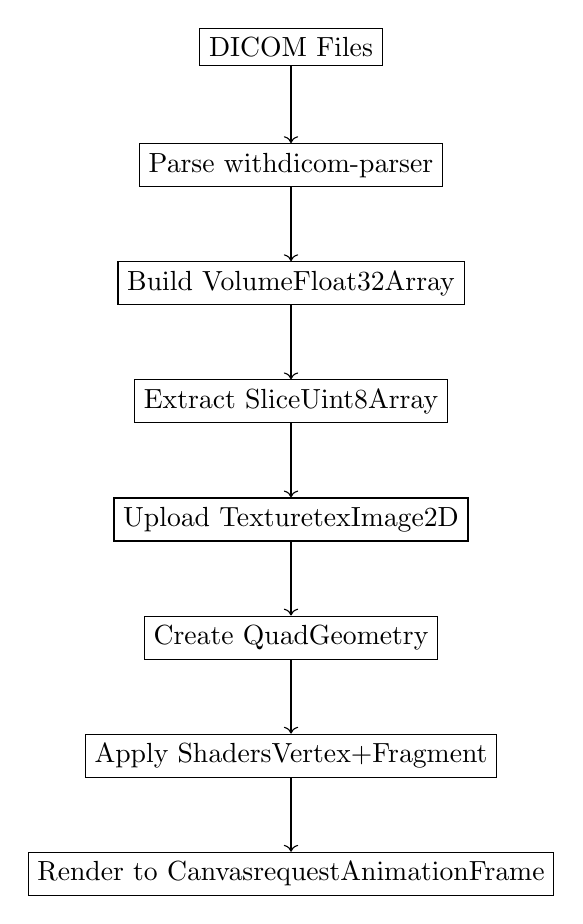
\begin{tikzpicture}[node distance=1.5cm, auto, scale=0.9]
  \node[draw, rectangle] (dicom) {DICOM Files};
  \node[draw, rectangle, below of=dicom] (parse) {Parse with\\dicom-parser};
  \node[draw, rectangle, below of=parse] (volume) {Build Volume\\Float32Array};
  \node[draw, rectangle, below of=volume] (slice) {Extract Slice\\Uint8Array};
  \node[draw, rectangle, below of=slice] (texture) {Upload Texture\\texImage2D};
  \node[draw, rectangle, below of=texture] (quad) {Create Quad\\Geometry};
  \node[draw, rectangle, below of=quad] (shader) {Apply Shaders\\Vertex+Fragment};
  \node[draw, rectangle, below of=shader] (render) {Render to Canvas\\requestAnimationFrame};
  
  \draw[->] (dicom) -- (parse);
  \draw[->] (parse) -- (volume);
  \draw[->] (volume) -- (slice);
  \draw[->] (slice) -- (texture);
  \draw[->] (texture) -- (quad);
  \draw[->] (quad) -- (shader);
  \draw[->] (shader) -- (render);
\end{tikzpicture}
\end{center}
\end{frame}

\begin{frame}
\frametitle{Key Technologies}

\begin{columns}
\column{0.5\textwidth}
\textbf{Frontend}
\begin{itemize}
  \item React + TypeScript
  \item Interactive UI controls
  \item Real-time slice selection
\end{itemize}

\textbf{Medical Data}
\begin{itemize}
  \item DICOM file format
  \item Multi-file volume assembly
  \item Hounsfield units
\end{itemize}

\column{0.5\textwidth}
\textbf{Graphics}
\begin{itemize}
  \item WebGL 1.0
  \item GPU texture storage
  \item Shader programming
\end{itemize}

\textbf{3D Math}
\begin{itemize}
  \item Matrix transformations
  \item Camera controls
  \item Orthogonal projections
\end{itemize}
\end{columns}
\end{frame}

\begin{frame}
\frametitle{Performance Characteristics}

\textbf{Memory Usage:}
\begin{itemize}
  \item Volume storage: $W \times H \times D \times 4$ bytes (Float32)
  \item Example: $512 \times 512 \times 200$ = 209 MB
  \item Texture: $W \times H$ (slice) = 262 KB
\end{itemize}

\vspace{0.3cm}

\textbf{Computational Complexity:}
\begin{itemize}
  \item Parse single DICOM: $O(n)$ bytes
  \item Build volume: $O(W \times H \times D)$
  \item Extract slice: $O(W \times H)$ or $O(W \times D)$
  \item Render frame: Real-time (GPU-accelerated)
\end{itemize}

\vspace{0.3cm}

\textbf{Optimizations:}
\begin{itemize}
  \item Lazy slice extraction (on-demand)
  \item GPU texture filtering (linear interpolation)
  \item requestAnimationFrame for efficient rendering
\end{itemize}
\end{frame}

\begin{frame}
\frametitle{Advantages of This Approach}

\begin{itemize}
  \item \textbf{GPU Acceleration}: Fast rendering of slices
  \item \textbf{Interactive}: Real-time slice navigation
  \item \textbf{Web-based}: No installation required
  \item \textbf{Standard Format}: Works with DICOM from any modality
  \item \textbf{Extensible}: Easy to add volume rendering, MPR, etc.
  \item \textbf{Cross-platform}: Works on desktop and mobile
\end{itemize}
\end{frame}

\begin{frame}
\frametitle{Future Enhancements}

\begin{itemize}
  \item \textbf{Volume Rendering}: Raycasting for 3D visualization
  \item \textbf{Windowing}: Intensity range control (Hounsfield units)
  \item \textbf{Measurements}: Distance, angle, area tools
  \item \textbf{Annotations}: Drawing tools for clinical notes
  \item \textbf{WebGL2}: Advanced shaders, compute
  \item \textbf{Multi-File}: Temporal sequences (4D)
  \item \textbf{Export}: Save processed images/videos
\end{itemize}
\end{frame}

\begin{frame}
\frametitle{Questions?}

\begin{center}
\Large
Thank you for your attention!

\vspace{1cm}

Code available at:\\
\texttt{github.com/rathoddinesh14/graphicus-harena}

\vspace{1cm}

Key Resources:
\begin{itemize}
  \item Khronos WebGL Specification
  \item DICOM Standard Documentation
  \item Medical Image Processing: Gonzalez \& Woods
\end{itemize}
\end{center}
\end{frame}

\end{document}
